\documentclass{article}
\usepackage[utf8]{inputenc}
\usepackage{graphicx}
	\DeclareGraphicsExtensions{.png, .jpeg}
\usepackage{caption}
% \usepackage{subcaption}
\usepackage[top=1in, bottom=1in, left=1in, right=1in]{geometry}

\title{Database Design and Implementation \\ HW 08}
\author{\underline{Team 08}\\Henriod, Terence\\Santoyo, Jorge \\Singh, Raja}
\date{\today}

\begin{document}

\clearpage
\maketitle
\thispagestyle{empty} % removes the page number from the title page

\begin{abstract} % Do we want to change this?
Create a logical ERD for each of the two questions in this document using the crowsfoot format discussed in class. Be sure that each entity has the entity name at the top of the box, the primary key attribute or attributes in the middle of the box, and the non-key attributes in the bottom of the box. Lines should separate each part of the entity box. The ERD should not have any M:N relationships and all attributes should be placed within an entity. Each entity must have a primary key defined. A primary key may consist of one or more attributes. Each relationship should have at least one relationship verb or verb phrase. Please include all required foreign keys and denote the foreign key(s) with the notation (FK) on the ERD.

You will turn in one copy of your ERDs at the beginning of class. This is the ``grading" copy. You will have another printed copy of your ERDs available for evaluation during class. If you are working in a group, please ensure that each group member has printed copies of the ERDs available for group work during class. Your group will not be working together during class, so each group member must have a printed copy of the group’s ERDs.

Please use Microsoft Visio or another computer-based diagramming tool for this assignment. Microsoft Visio is available in the College of Business computing labs. It can also be downloaded for free from DreamSpark. We reviewed the functions of Microsoft Visio 2010 in class.
\end{abstract}
%
%
%
\newpage
\section{Exercise 01: Board Game Company Database}
Design a database to store data for orders placed by customers. The company requesting this database uses the web as a platform to sell physical board games directly to the public. The ``order form" included as Figure 1 shows the data used during the ordering process, but of course the company has very pretty graphical forms on its web site. The structure of the form does not affect the design of the database. You can assume the following about the ordering process in this organization:
\begin{itemize}
  \item Orders are placed over the web or by telephone. The data on the order form in Figure 1 is captured when an order is taken.
  
  \item The company does not capture credit card data in this database – that information is stored within the billing database, which is not within the scope of your design.
  
  \item The company stores the address information for a customer as part of the customer information. Customers are kept on file whether or not there is a current order for a customer. It is possible for a customer to have more than one order on file, but each order is for one and only one customer. There is only one customer address per customer.
  
  \item There is only one shipping address per order. (Note: we will discuss in class how the design must change to accommodate multiple shipping addresses per order.)
  
  \item The shipping address may differ from the customer address.
  
  \item Each order consists of one or more games. Each game can be on zero or more orders.
  
  \item The price for a game is the same for every order. The price is not calculated – it is associated with the game.
  
  \item The extended price, shipping cost, discount amount, and order total are all calculated fields.
  
  \item The discount code and credit code attributes have the potential to be different for each order for a given customer. There is only one discount code and one credit code per order.
  
  \item Each game on an order may have a different quantity ordered. In Figure 1, the customer ordered a quantity of one for GameID A10012, but ordered a quantity of two for GameID B23009.
  
  \item Each game on an order may have a different estimated shipping date. The estimated shipping date is related to a game on an order.
\end{itemize}
After an order is placed, the company ships the game(s) to the customer. The data on the shipping form included as Figure 2 is captured when the company ships the game(s) to a customer. Here is some information about the shipping process:

\begin{itemize}
  \item Games are shipped from a variety of different warehouse locations around the world to customers. Each location is identified by its locationID. The company keeps track of the name of the warehouse at the location. A given locationID has only one warehouse name associated with that location.
  
  \item The company may receive an order for a quantity of two for the same game, as shown in the sample order, but then actually ship that same game from two different locations, as shown in the two sample shipping forms. The final shipping quantity is accurate in this example, but the company needed to ship from two different warehouse locations. Thus, a game on an order may have a minimum of zero shipments associated with it, or may have multiple shipments associated with it. There will be a unique tracking number for each shipment made.
  
  \item A shipment may consist of more than one game on an order, as shown in shipping form example \#1, however, there will only be one order affiliated with a given tracking \#. A unique tracking number is always generated for a different order.
  
  \item The actual shipping date may differ from the estimated shipping date. The company wants to store both the actual and estimated shipping date in this database.
  
  \item The company may make a partial shipment (ex: ship only 1 game when the order calls for 2 of the same game; another ex: ship 2 of the games on an order and delay shipment of the third game).
  
  \item The company may accidentally overship a game (ex: the order says that a quantity of 2 is ordered, but the company accidentally ships 3). The company wants to keep track of the quantity shipped of each game on each purchase order.
  
  \item The database should not prevent partial shipments or overshipments – these are simply circumstances that may happen and are acceptable business rules.
\end{itemize}

\begin{figure}[h!]
  \centering
  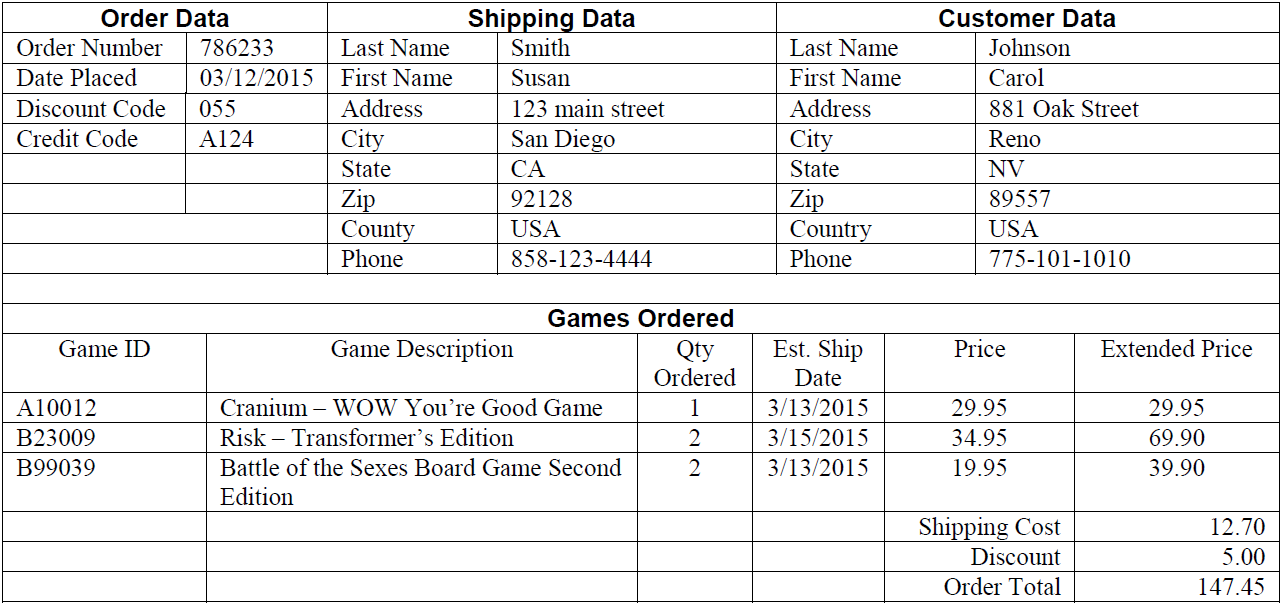
\includegraphics[width=.75\linewidth]{HW08_Ex01_order_form}
  \caption{An example of an order form for ordering board games.}
  \label{fig:HW08_Ex02_order_form}
\end{figure}

\begin{figure}[h!]
  \centering
  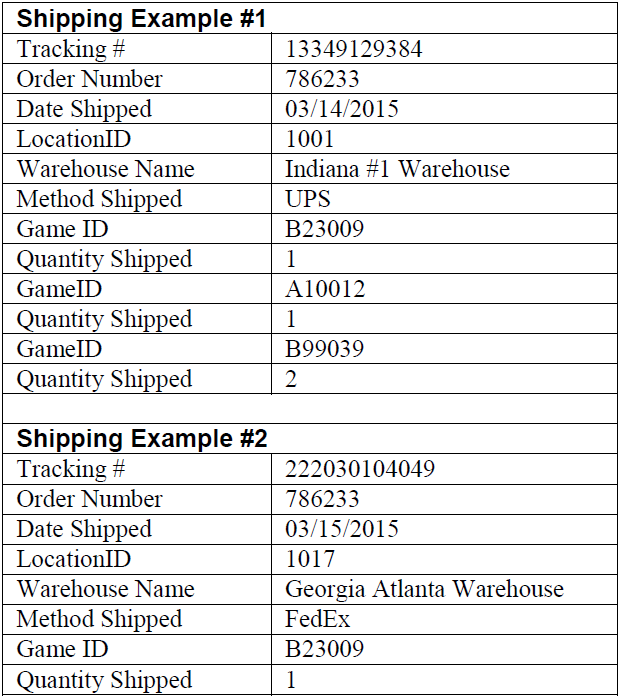
\includegraphics[width=.35\linewidth]{HW08_Ex01_shipping_form}
  \caption{An example pair of a shipping information form for shipping board games.}
  \label{fig:HW08_Ex01_order_form}
\end{figure}

\newpage
\textit{Solution}:\\

  \begin{figure}[h!]
    \centering
    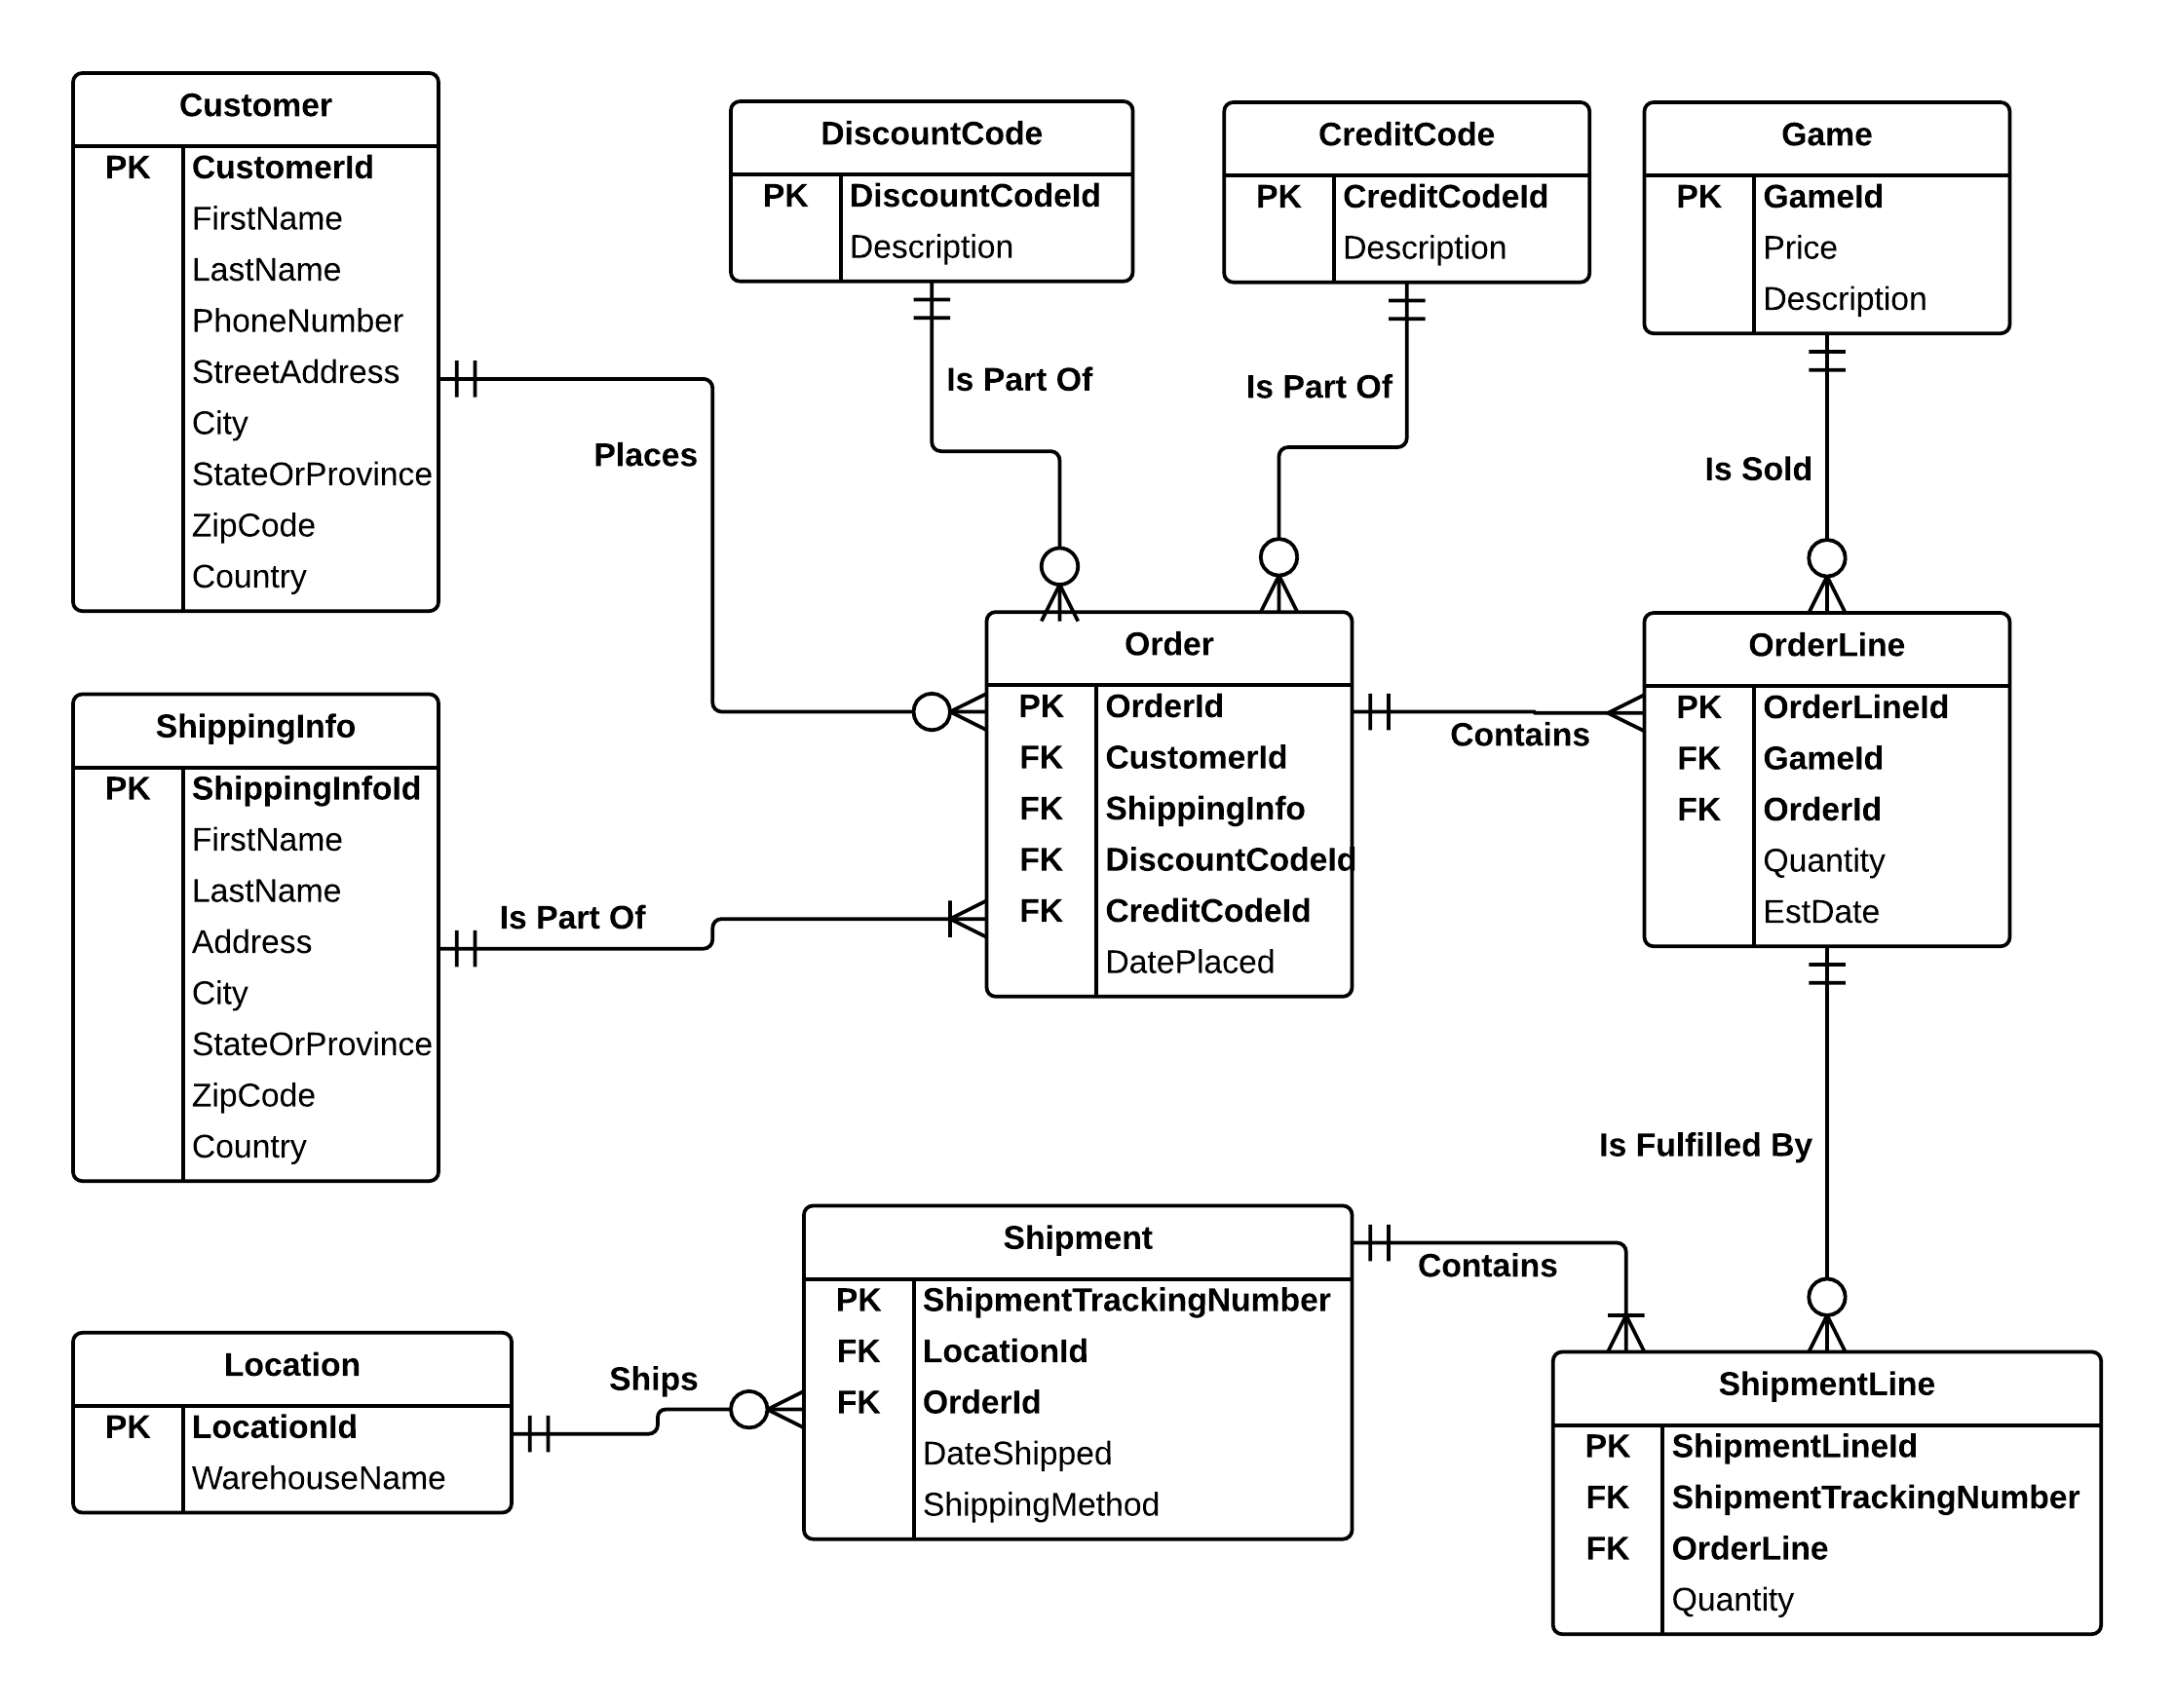
\includegraphics[width=.95\linewidth]{HW08_Ex01_solution_ERD}
    \caption{The solution ERD for the board game vending company's database.}
    \label{fig:HW07_Ex01}
  \end{figure}
Assumptions:
\begin{itemize}
  \item Discount and Credit codes may be created, but never used.
  \item There may not be any shipments for an order line in the case that an item is on back-order and the stock is never replenished.
  \item A customer may never place an order, but may be a customer in terms of having built an on-line shopping cart or receives promotional information.
  \item Some (bad) games may never be sold (not even once!).
\end{itemize}
%
%
%
\newpage
\section{Exercise 02: University Student Information Database}
Imagine that a university generates a student information screen (Figure 3) that consolidates grade data for a given semester along with basic data about that student. This screen may be viewed by a student or an advisor at a university. The goal of this exercise is to design a database that will support the production via SQL of the grade screen shown in Figure 3, as well as store the additional data discussed in the business rules below. The student information screen would be produced by SQL queries from the database you design.
The relevant business rules for this database are:
\begin{enumerate}
  \item A course is uniquely identified by a course ID. The course ID determines the title of the course.
  
  \item A student is uniquely identified by a student ID.
  
  \item The school uses a semester system. All courses are identified by when they are taken: semester (Fall, Spring, Summer 1, Summer 2, Interim 1, Interim 2) and year. For example, a course taken in the Spring 2015 semester would be listed as S2015 while a course taken in the Wintermester session of 2015 would be listed as WIN2015. The database must be able to differentiate among classes taken in different semesters/sessions of different years.
  
  \item The ``year" of a student (sophomore, junior, etc.) is determined based on the total number of credits completed by that student.
  
  \item A student can take a class more than once. For example, it is possible that the student in Figure 3 took BIOL 316 in a prior semester. The university keeps track of all times that a student has taken a course, along with whatever grade the student earned for that course. This database should keep track of all the semesters that a student has taken a course, and the resulting grade.
  
  \item A student can, theoretically, take an unlimited number of courses each semester. However, a student can take a specific course (like ACC402) only once per semester.
  
  \item Only one instructor teaches each section of a course. There are no team-teaching sections of courses.
  
  \item There may be more than one section of a given course offered in a semester. It is possible that different instructors will teach different sections of a course. For example, it is possible that there are three sections of BIOL316. One instructor may teach two sections and a different instructor teaches the third section. It is OK to include a section number as an attribute in this database design; a section number is a natural attribute in this system, even though it isn’t shown in Figure 3. Section numbers, however, do not make a course unique. Examples of section numbers are 1001, 1002, 1003. For example if there are three sections of BIOL316, then they would be labeled BIOL316-1001, BIOL316-1002, BIOL316-1003 with their respective section numbers.
  
  \item A specific section of a specific course will be uniquely identified by a number when this database is physically implemented. For the logical model you are creating, think about what attributes you could concatenate to uniquely identify a section of a course taught during a semester of a year.
  
  \item The university would like to keep track of course prerequisites in this database. A course can have zero or many prerequisites. A could could serve as the prerequisite for zero or many other courses.
  
  \item The number of credits for a course depends on the student taking the course. For example, it is possible that a student can take an information systems internship (IS480) for 1, 2, or 3 credits. The specific number of credits that a student takes for a course would be stored with the student-course data. The university, however, would also like to keep track of the default number of credits for which a course is offered. For example, the default number of credits for IS480 is 3. The default number of credits should be stored with the course data.
  
  \item Assume that you are designing a database for only one campus of one university. The university is subdivided as follows: The university is divided into colleges and the colleges are divided into departments. A department must be affiliated with a college. Departments offer majors and minors; all majors and minors must be offered by a department. For example, the College of Sciences is divided into many departments, one of which is Biology. The Biology department offers majors in biology, biological engineering, entomology, etc. The Biology department offers minors in some of the same fields. For example, the Biology department offers both a major and a minor in Biology and Biological Engineering. The College of Liberal Arts also offers many majors such as Psychology, English, Philosophy, Political Science, etc. A given department is only in one college.
  
  \item A college has unique majors and minors that are not offered by any other colleges. For example, the College of Sciences houses the botany major of the student on the screen shown in Figure 3. There are no other ``colleges" at the university that house botany majors. A given major is offered by only one department. A given minor is offered by only one department.
  
  \item A student can have multiple majors and minors. A student does not have to have either a major or a minor.
  
  \item A student’s ``College Affiliations" is based on the placement of the major and/or minor. In Figure 3, the student is majoring in Botany, so that college affiliation is with the College of Sciences. She is minoring in Accounting, so that college affiliation is with the College of Business. She is also minoring in Psychology, so that college affiliation is with the College of Liberal Arts. See bullet point \#12 for information about how majors are related to colleges at the university.
  
  \item This database does not keep track of the classes that compose a given major or minor.
\end{enumerate}
\textbf{Important issue for design:} A key point to think about is: what will it take to uniquely identify a student’s grade for a specific course taken during a specific semester of a specific year. Keep in mind that a student can easily take the exact same course more than once and the grade will be stored as many times as the student takes the course – the grade will not be over-written (they will not use the SQL UPDATE command to overwrite the grade, they will use the SQL INSERT command to add another row in the table where the grade is stored) in the database.

\begin{figure}[h!]
  \centering
  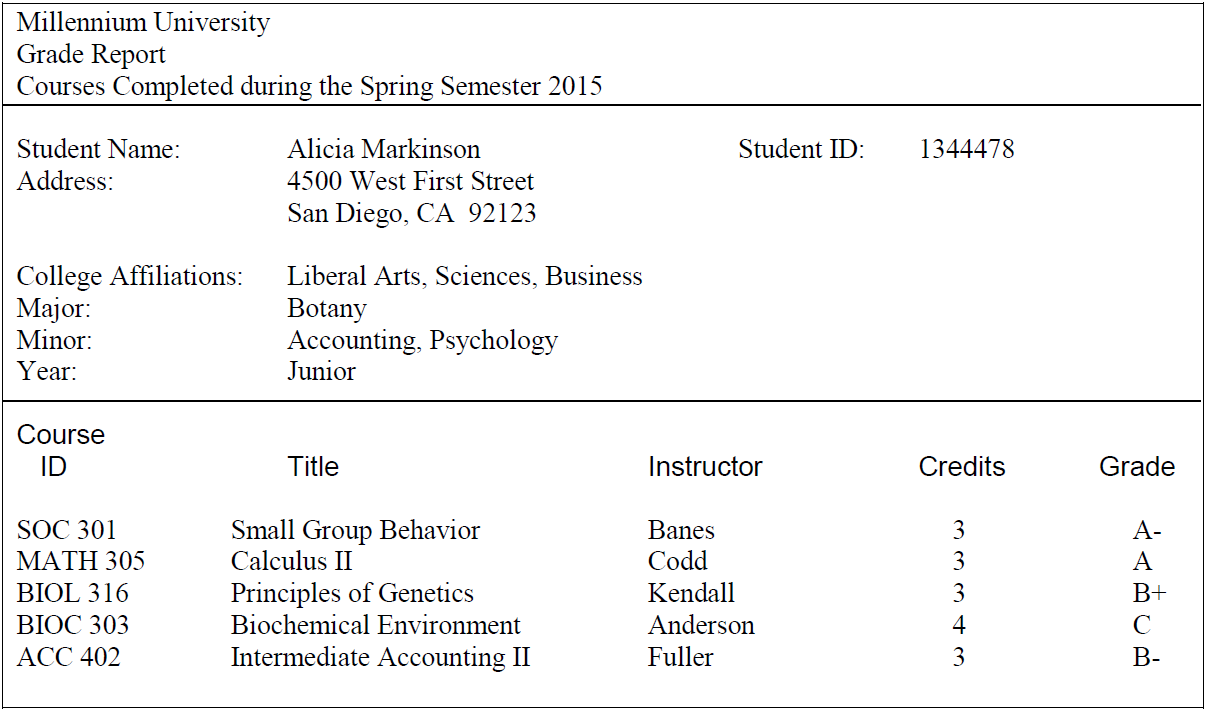
\includegraphics[width=.65\linewidth]{HW08_Ex02_student_info_screen}
  \caption{An example screenshot of a student's information as the system should produce it.}
  \label{fig:HW08_Ex01_order_form}
\end{figure}

\newpage
\textit{Solution}:\\

  \begin{figure}[h!]
    \centering
    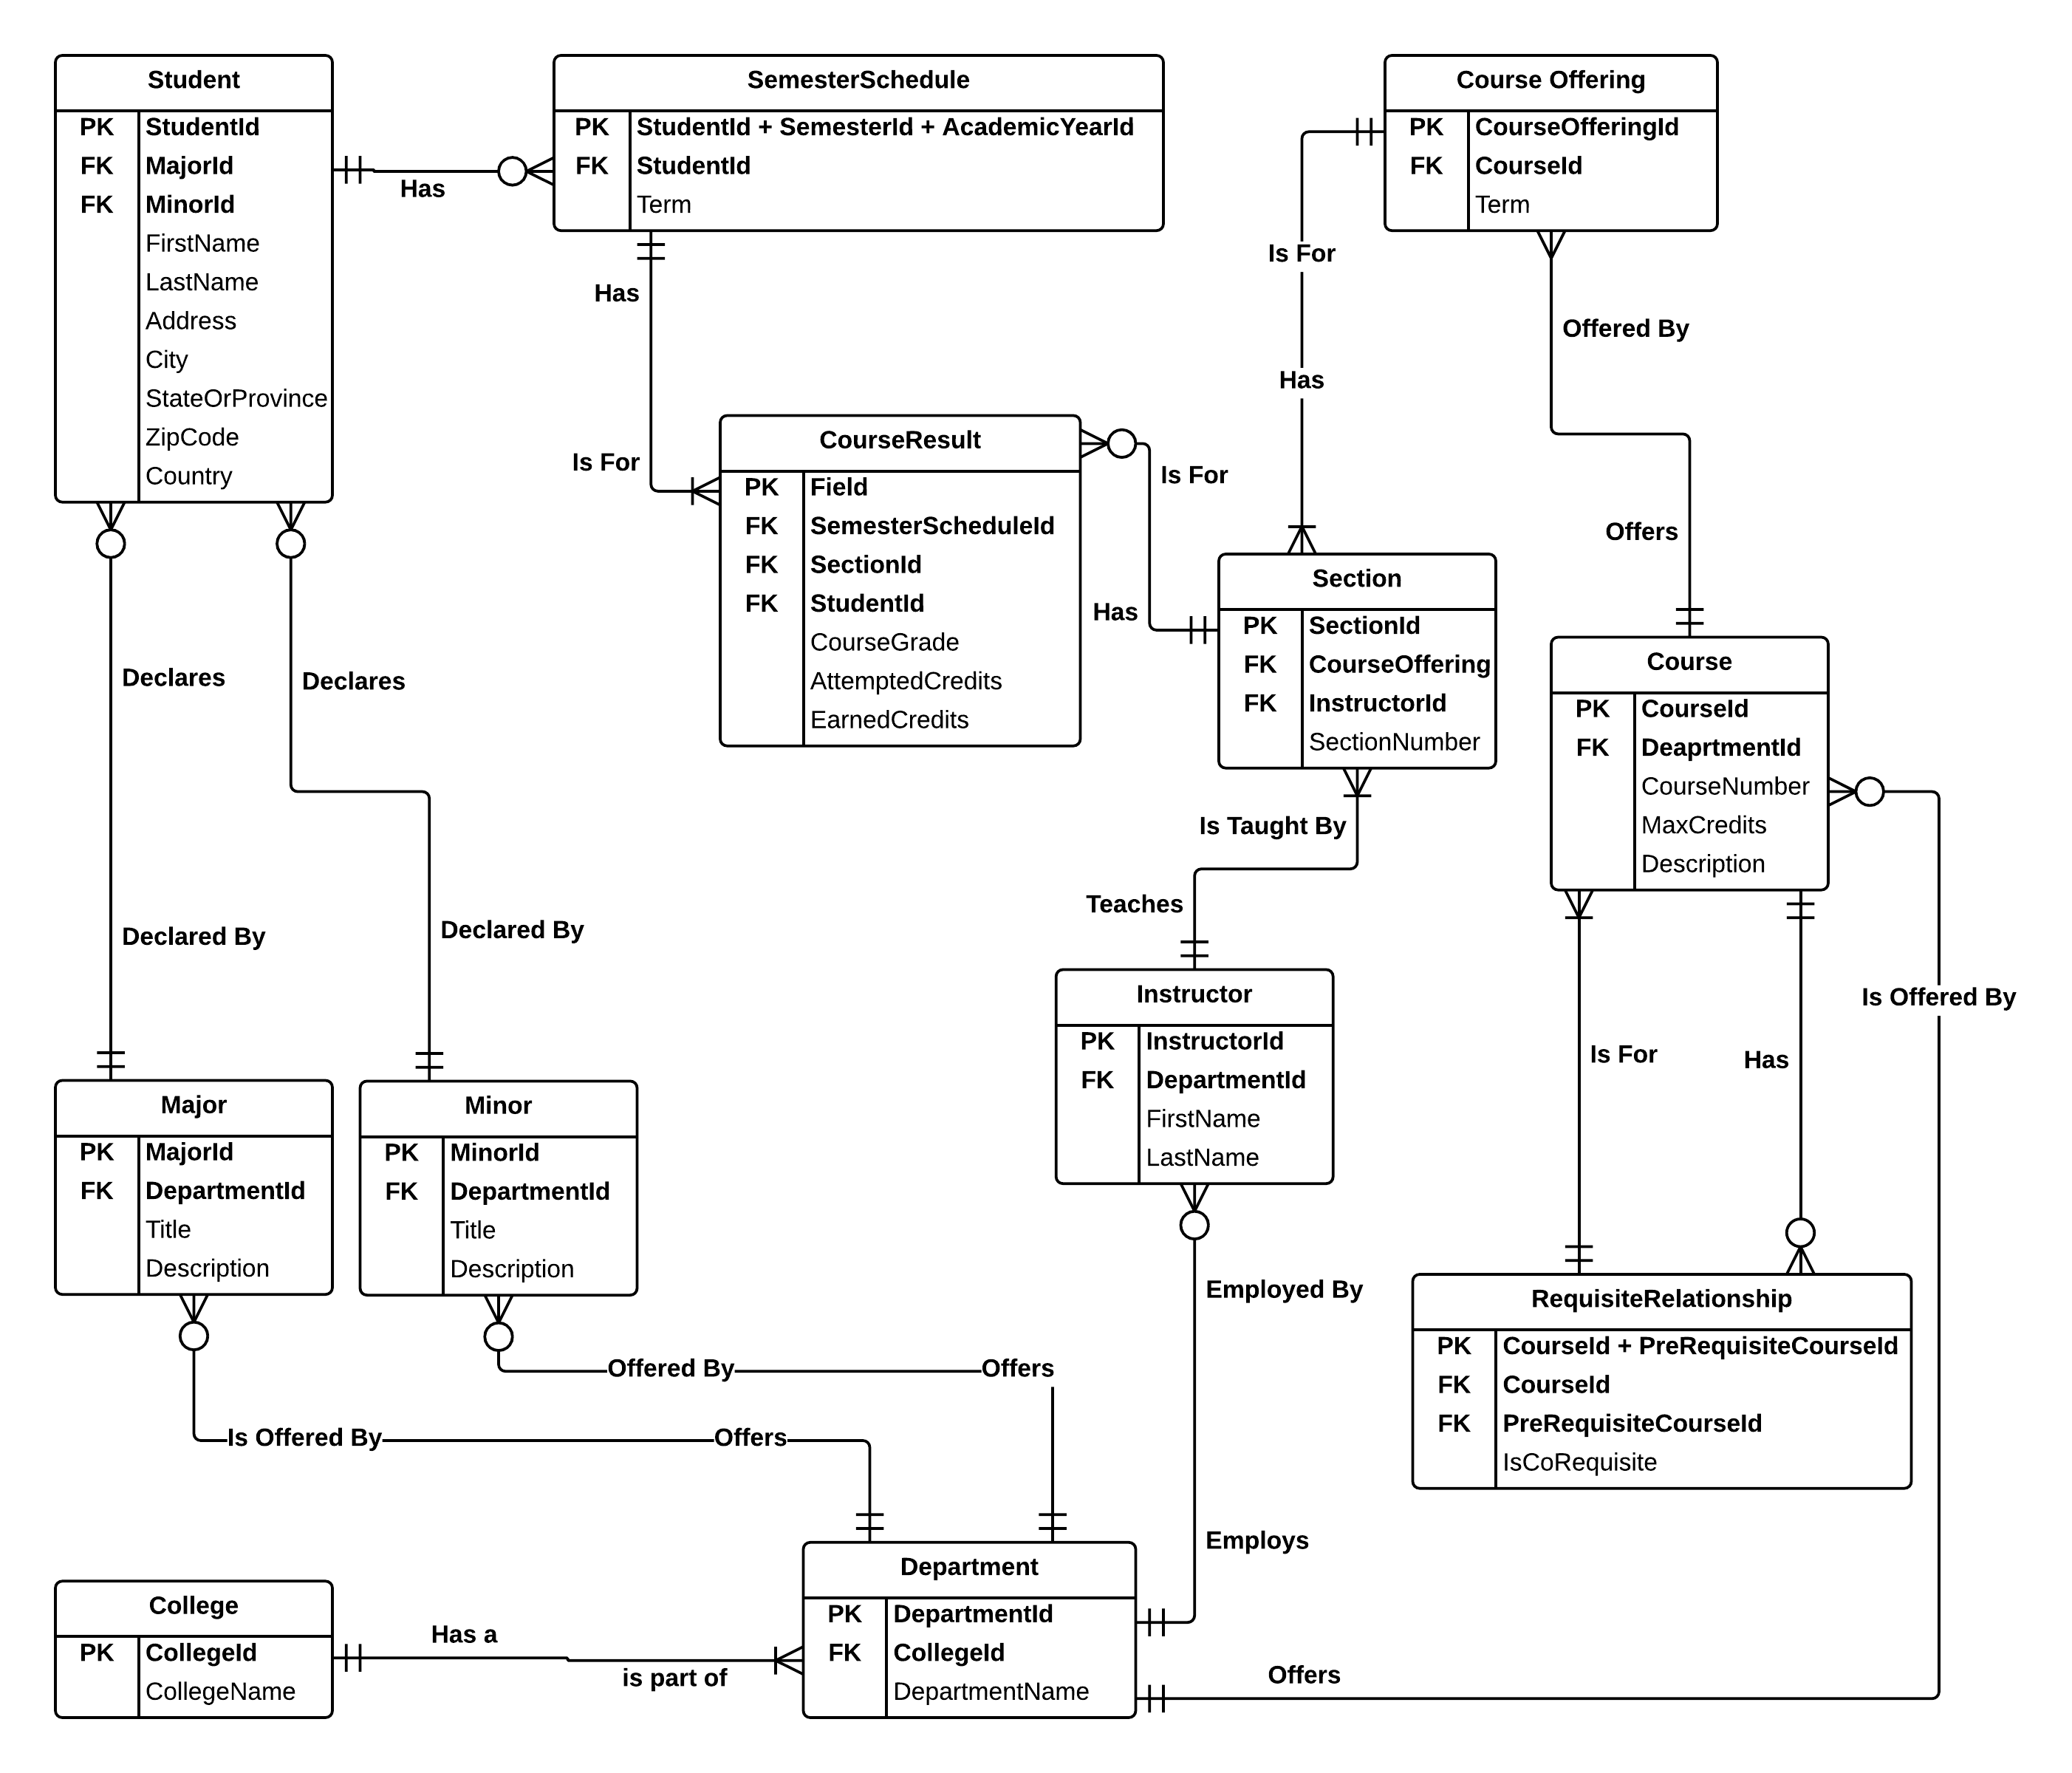
\includegraphics[width=.95\linewidth]{HW08_Ex02_solution_ERD}
    \caption{The solution ERD for the college's student information database.}
    \label{fig:HW07_Ex02}
  \end{figure}
Assumptions:
\begin{itemize}
  \item The problem statement defines a business rule that states that a student cannot have a course multiple times on a given semester's schedule. We feel that this is not a data model design's problem to handle, this is something that should be handled on the front-end through appropriate queries to check if an action is allowable or not.
  \item We assume it is possible that no students sign up for a section(s) of a course.
  \item The line between pre-requisite and co-requisite is fine.
  \item There can be (specialized) colleges/departments that do not offer majors/minors or courses and such.
  \item A student can enroll before having an official semester schedule.
  \item The \texttt{CourseResult} entity will hold the status of a current course until a final grade is posted.
\end{itemize}

\end{document}